\section{\texorpdfstring{Zásobník - paměť STACK}{Zasobnik - pamet STACK}}

% =====================================================================================================================
	\begin{frame}
    \frametitle{Co je zásobník?}
		\small
		\begin{itemize}
			\item speciální část paměti \textbf{RAM} fungující jako struktura \textbf{LIFO},
			\item \textbf{L}ast \textbf{I}n, \textbf{F}irst \textbf{O}ut: poslední zapsaná data jsou jako první vyčtena,
			\item na vrchol zásobníku ukazuje \textbf{S}tack \textbf{P}ointer (\textbf{SP} = registr ukazatele),
			\item vrcholem se rozumí první neobsazené místo paměti,
			\item vrchol prázdného zásobníku je na nejvyšší adrese, plněním tak \textbf{SP} ukazuje stále na nižší adresy,
		\end{itemize}
		
		\vspace{3mm}
		\begin{center}
			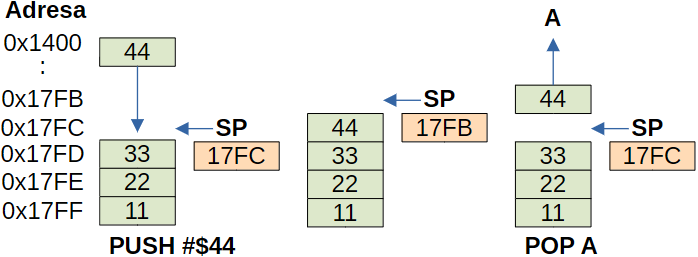
\includegraphics[width=0.80\textwidth]{fig/stack.png}
		\end{center}
		
	\end{frame}

% =====================================================================================================================
	\begin{frame}
    \frametitle{K čemu se zásobník používá?}
		\small
		\begin{itemize}
			\item ukládají se do něj návratové adresy funkčních skoků:
			
			\begin{itemize}
				\item \textcolor{blue}{\textbf{CALL}}: do zásobníku uloží adresu následující instrukce a skočí na návěstí,
				\item \textcolor{blue}{\textbf{RET}}: ze zásobníku přečte adresu a skočí na ni.
			\end{itemize}
			
			\item ukládají se do něj návratové adresy přerušení a záloha systémových registrů,
			\item ve funkcích do něj ukládáme (vytváříme) lokální proměnné.
			
		\end{itemize}
		
		\vspace{1mm}
		\begin{center}
			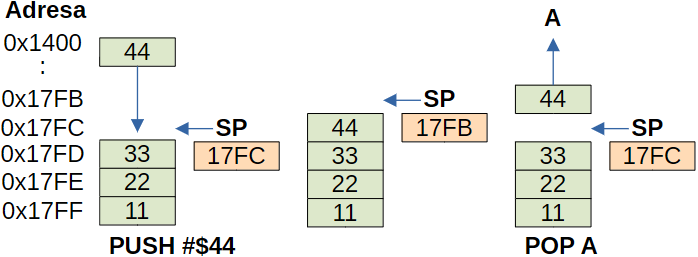
\includegraphics[width=0.80\textwidth]{fig/stack.png}
		\end{center}
		
	\end{frame}
	
% =====================================================================================================================
	\begin{frame}
    \frametitle{Indexová adresace zásobníku}
		
		\textbf{Příklad:} \textcolor{blue}{\textbf{LD}} A, (\$03, SP) \textcolor{teal}{; SP = první neobsazená adresa}
		\small
		\begin{center}
			\begin{tabular}{c | c}
				\textbf{Před výkonem instrukce} & \textbf{Po vykonání instrukce} \\ \\
				
				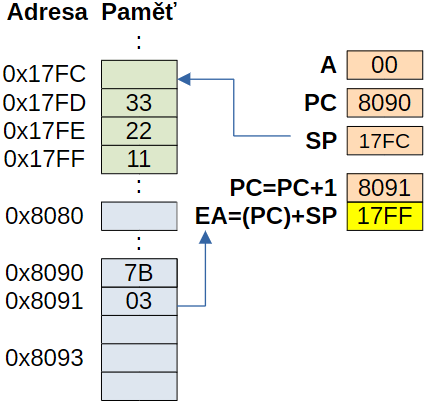
\includegraphics[width=0.45\textwidth]{fig/indexova_adresace_stack.png} & 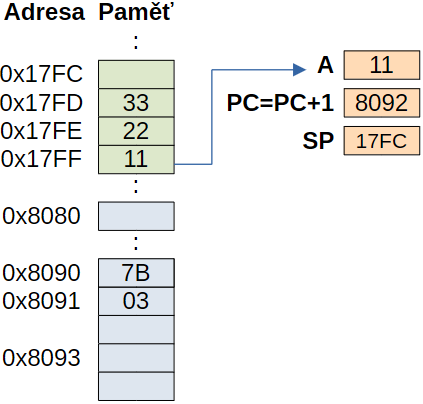
\includegraphics[width=0.45\textwidth]{fig/indexova_adresace_stack_po.png} \\
				
			\end{tabular}
		\end{center}

	\end{frame}